\chapter{Species trait prediction via phylogenetic latent factors}
\chapterauthor{Maxwell B. Joseph, Kevin B. Knight, Pieter T. J. Johnson}

As trait-based approaches in ecology have gained momentum, efforts to assemble trait databases have increased the availability of trait data for many taxa.
However, observations are often missing from these databases, and species with incomplete trait records may be excluded from analyses, thereby limiting the utility of trait-based approaches and potentially biasing subsequent inference.
Here we develop a hierarchical Bayesian method to interpolate missing traits, exploiting correlations among traits and phylogenetic autocorrelation.
The model maps observable traits to phylogenetically structured latent factors.
We demonstrate this approach on a database of primate species traits with K-fold cross validation to approximate out-of-sample predictive power for models with varying latent factor dimensionality and phylogenetic correlation structure.
The expected and predicted values were highly correlated with the held-out values (r = 0.86 and 0.79, respectively), and 95\% of the 95\% prediction intervals contained the true trait value.
This latent factor approach provides a means to interpolate missing observations in species level trait databases, particularly for poorly described species with well described evolutionary neighbors.
We conclude with some promising applications for estimating extinction risk, along with methodological extensions to this latent factor approach.


\section{Introduction}

In recent decades, many species trait databases have been assembled to meet the needs of trait-based approaches, which rely on species traits to achieve a more quantitative understanding of ecological phenomena, rather than simply treating species as categorically different \citep{Ackerly2007, Gross2009, Webb2010}.
In the process of constructing trait databases, some entries (trait-by-species combinations) may be missing because no records for a trait are available for a species, and this raises issues with inclusion/exclusion rules for species in an analysis \citep{Nakagawa2008}.
This problem is compounded when trait databases include many traits or poorly sampled species.
These missing data are problematic for trait-based approaches in the same way that missing covariates are generally problematic in statistical modeling \citep{little2014statistical}.

One solution to this missing data problem lies in interpolating missing trait values.
Information on missing traits can be derived from closely related species if traits show phylogenetic autocorrelation - that is, if closely related species tend to have similar trait values \citep{Felsenstein1985}.
While phylogenetic non-independence can be a nuisance for many comparative analyses because it violates common assumptions of conditional independence, in the context of trait interpolation it is an asset.
Indeed, existing trait interpolation methods such as phylogenetic eigenvector mapping (PEM) make use of phylogenetic autocorrelation to acquire informed estimates of species traits, thereby helping to overcome potential biases in species inclusion \citep{Guenard2013}.
Information can also come from other correlated traits recorded from the same species \citep{Westoby2002, Poorter2006, Zheng2009}.
For instance, large-bodied mammals tend to reproduce more slowly; thus, for a newly described large mammal with no recorded reproduction data, we would expect a long gestation period \citep{Promislow1990}.
Our confidence in this prediction will depend on the strength of correlation between the traits.
Prediction uncertainty is inherent to interpolation, and ideally this uncertainty would be propagated forward through an analysis that makes use of interpolated traits.

Here, we present a hierarchical Bayesian method for missing-trait interpolation that makes use of latent, life history factors that are structured phylogenetically.
This method exploits information from closely related species and from correlated traits to acquire the full posterior distributions for missing traits, conditional on the observed traits.
The acquisition of a posterior distribution for missing traits facilitates error propagation, incorporating uncertainty in the model parameters in trait interpolations.
This approach simultaneously uses both incomplete and redundant traits with no requirement that any trait be observed for every species \citep{Guenard2013}, thereby expanding its utility to a wide range of situations.
Using trait data from 168 primate species, we illustrate the efficacy of this model in predicting unobserved trait values.
We conclude with a comparison to existing trait imputation methods, and suggest some future applications and extensions to improve the utility of these approaches.

\section{Methods}

\subsection{Data description}

We compiled primate species trait data from multiple sources, including the Handbook of the Mammals of the World, the PanTHERIA database, and a recently published dataset of species traits for amniotes \citep{myhrvold2015}.
We obtained a phylogenetic tree of 346 primate species from \cite{perelman2011}, and of these, 168 species were represented in the trait data.
After subsetting the trait data to species in the phylogeny, all species traits were logarithm(+1) transformed, centered, and scaled to have mean zero and unit standard deviation.
The resulting dataset was a trait matrix with 168 species (columns) and 22 traits (rows), available in the data supplement.
In this matrix, 36.4\% of trait observations were missing overall (Figure \ref{fig:missingness}).
No single trait was completely observed, with the percentage of missing data for traits ranging from 0.6\% to 77.8\%.
Further, there were no species with complete trait observations, with the percentage of missing observations at the species level ranging from 9.1\% to 95.4\%.

\subsection{Model structure}

The aim of our modeling approach was to predict missing species-trait data using incomplete information for a species, as well as any information from closely related species.
To achieve this goal, we developed a model that is similar to factor analytic models, where observed data are treated as random variables that are functions of latent factors. In turn, each of these latent factors has some loading coefficient determining the effect on the observed variable \citep{Lopes2004}.
For traits $i=1,..., N$ and species $j=1,..., J$ any particular trait observation is $z_{ij}$, making up the elements of $Z$ which represents the trait matrix.
Define $y_{ij}$ to be the transformed trait value, which has undergone a log(+1) transformation, followed by centering and scaling for each trait.
These traits make up the elements in an $N$ by $J$ matrix $Y$, which contains the transformed trait values.
If there are $M$ latent factors, where $M < N$ then each species $j$ is associated with a vector $f_{.j} = (f_{1j}, f_{2j}, ..., f_{Mj})^T$ of species-specific latent factor values, where the dot subscript in $f_{.j}$ indicates all of the elements across the first index.

To make use of phylogenetic information, we assumed that these latent factors covaried among species, and borrowed ideas developed for spatially autocorrelated factor analysis to allow for phylogenetic autocorrelation \citep{Hogan2004}.
We assumed that the latent factors would be correlated among species, but uncorrelated among each other.
We defined a vector of latent factor values for each species $j=1, ..., J$, corresponding to each of the $M$ latent dimensions, and imposed a mean zero Gaussian process prior on the vector such that $f_{m.} \sim GP(0, K(d))$, where $K(d)$ is a decreasing covariance function of cophenetic distance $d$, the pairwise distance between species in the phylogenetic tree, so that closely related species may have more similar latent factor values than distantly related species \citep{Neal1998}.
This implies a multivariate normal prior on all of the latent factors concatenated into vector: $vec(f) = (f_{1.}^T, f_{2.}^T, ..., f_{M.}^T)^T$, and $vec(f) \sim N(0, \Sigma)$, where $\Sigma$ is a block diagonal covariance matrix with $M$ blocks, each being a covariance matrix with potentially varying parameters obtained by applying the correlation function $K(d)$ to an $N$ by $N$ square matrix $D$ that contains the cophenetic distances among species obtained from the phylogenetic tree.
Fixing the variance of each latent factor to equal one - a common identifiability constraint - the covariance function effectively becomes a correlation function \citep{Shapiro1985}.

We considered five correlation functions that varied in their assumptions about the correlations in latent factors as a function of phylogenetic distance (Figure \ref{fig:cor_functions}).
Some of these functions such as the exponential allow for long range phylogenetic dependence, while others such as the spherical limit long range dependence.
The absence of phylogenetic autocorrelation is represented with a phylogenetically independent correlation function $K_{indep}(d) = I_{d = 0}$, which returns an $N$ by $N$ identity matrix for any cophenetic distance matrix $D$.
Theory suggests that multiple phylogenetic correlation functions can result from different mechanistic models of evolution \citep{Hansen1996}, but here the goal is simply to interpolate traits, not to represent explicit models of evolution.

Traits arise from the latent factors with process and measurement error.
To map the $N$ measured traits to the $M$ latent factors, we use a rectangular loading matrix $\Lambda_{N \times M}$.
The upper triangular elements of $\Lambda$ are fixed at zero, and the diagonal elements $(\lambda_{11}, \lambda_{22}, ..., \lambda_{DD})$ are positive, ordered, and decreasing \citep{West2003, Conti2014a}.
We used a lognormal prior on the diagonal elements to avoid diagonal loadings of zero, with mean zero and unit variance, and a normal prior on the remaining elements: $\lambda_{im} \sim N(0, \sigma_\lambda): i \neq m$.
Here $\sigma_\lambda$ is a hyperparameter that controls the variation in non-diagonal loadings, and it received a half-Cauchy prior: $\sigma_\lambda \sim Cauchy_{+} (0, 5)$.
A matrix $F_{M \times J}$ contains the latent factor values such that element $F_{m, j}$ corresponds to latent dimension $m$ and species $j$.
The $N$ by $J$ matrix product $\Lambda F$ provides the mapping of latent factors to the observations.
We also included parameters for the means $\alpha_1, ..., \alpha_N$ and variances $\sigma^2_1, ..., \sigma^2_N$ for each trait, although we expected these to be close to zero and one respectively after centering and scaling the data.
Therefore, we used informative normal priors centered around zero for the means $\alpha_i \sim N(0, 0.1)$, and informative half-Cauchy priors for the standard deviations $\sigma_i \sim Cauchy_{+} (1, 0.1)$.
For notational convenience, we also define a matrix $A_{N \times J}$, with the $(i, j)^{th}$ element $\alpha_{ij} = \alpha_i$.
Then the model can be written compactly as $Y = \Lambda F + A + \epsilon$, with $\epsilon_{N \times J}$ being a matrix of normal residuals with trait-specific distributions: $\epsilon_{ij} \sim N(0, \sigma_i)$.

We assumed that traits were missing completely at random - that is, the presence or absence of an observation was independent of its value \citep{little2014statistical}.
This assumption may be violated if for instance, smaller species are harder to measure, such that missing body mass observations are a non-random sample of the body mass distribution.
If there were known missingness mechanisms, they could be modeled, with the potential to increase the precision with which missing traits are predicted \citep{Reich2010}.

\subsection{Parameter estimation}

We used automatic differentiation variational inference, implemented via the Stan probabilistic programming language, to approximate the posterior distribution of the parameters \citep{Hoffman2014, Kucukelbir2015} \nocite{stan-software:2015}.
This algorithm is considerably faster than traditional Markov chain Monte Carlo methods, allowing us to estimate parameters for many models with a relatively large dataset in $\approx$ 48 hours on a 4-core laptop.

\subsection{Evaluating predictive performance}

We used K-fold cross validation to compare the predictive power of the models in our model set, which included models with the five different latent factor correlation functions, and up to 17 latent factor dimensions \citep{Arlot2010}.
Each observation was assigned to one of $K=10$ folds at random, generating $K$ test data sets $y_k$, with $k = 1, ..., K$.
For any fold, the observations not assigned to that fold comprise a training data set, $y_{-k}$, which is used to obtain a posterior distribution for the parameters $p(\theta \mid y_{-k})$.
Predictive performance for observation $i \in k$ is quantified as the log predictive density, averaging over $S$ posterior simulation draws: $\widehat{lpd}_i = log(S^{-1} \sum_{s=1}^{S} p(y_i \mid \theta_{k,s}))$ \citep{gelman2014}.
If $\widehat{lpd}_i$ is high, then $y_i$ is predicted well by the model.
For each model, we obtained a summary measure of predictive performance by summing over $N$ to obtain the expected log predictive density $\widehat{elpd} = \sum_{i = 1}^N \widehat{lpd}_i$ \citep{Vehtari2015a}.
To calculate uncertainty in model performance, we also calculated the standard error of the expected log predictive density $se(\widehat{elpd}) = \sqrt[]{N var(\widehat{elpd})}$, where $var$ is the sample variance function computed over all observations $i = 1, ..., N$.

\section{Results}

In predicting unobserved traits among the included primate species, the model with a squared exponential correlation function and seven latent factors exhibited the highest predictive performance (Figure \ref{fig:model_comparisons}).
For this model, posterior trait expected values correlated strongly with the held-out test values with the median correlation coefficient $r_{med} =$ 0.856, and 95\% posterior credible interval (CI): (0.802, 0.905).
In addition, the posterior predicted trait values - which include both inferential and predictive error - also were well-correlated with the held-out values, with $r_{med}=$0.793 and CI: (0.675, 0.854)  (Figure \ref{fig:rho}).
Interval coverage was as expected with 95\% of the 95\% posterior prediction intervals containing the true trait values (Figure \ref{fig:predictions}).
While the squared exponential, seven-factor model performed best, other models with exponential and rational quadratic correlation functions were also well supported, whereas both the phylogenetically independent and spherical correlation function models performed poorly (Figure \ref{fig:model_comparisons}).

Predictive performance was best for traits that were well sampled, while traits with few data points had higher predictive error (Figure \ref{fig:mse}).
The most poorly sampled traits, such as the lower and upper bounds on body height, were predicted rather poorly, and should be taken with skepticism (Figure \ref{fig:by_trait}).
Predictions for these traits varied little, being closely centered around the mean values, and also showed low precision, with wide posterior credible intervals, unlike predictions for the well-sampled traits (Figure \ref{fig:by_trait}).

\section{Discussion}

By taking advantage of incomplete trait records and phylogenetic autocorrelation, the latent-factor approach developed here facilitated estimation of missing species traits and performed well based on cross validation.
The most well-supported model made use of a squared exponential phylogenetic correlation function for the latent factors, for which closely related species are very similar, and distantly related species are dissimilar.
In contrast, the model with no phylogenetic structure showed poor predictive performance (Figure \ref{fig:model_comparisons}).

In addition to acquiring estimates of missing species traits, this method also offers insights about which latent factors are correlated among species, but uncorrelated across the $M$ latent dimensions.
These latent factors could be used as explanatory variables for other species-level characteristics, including estimates of extinction risk, and may outperform species traits in this regard because they are uncorrelated with each other, resulting in less variance inflation for coefficient estimates \citep{Stine1995}.
In particular, this approach could prove useful for data-deficient species with well-described phylogenetic neighbors that provide information on the poorly sampled species' latent factor values \citep{Morais2013}.

This Bayesian latent factor approach has some potential advantages and disadvantages compared to existing phylogenetic trait interpolation methods.
Compared to phylogenetic eigenvector mapping, which uses phylogenetic topology and branch lengths to predict missing species traits one at a time, this method operates on all traits simultaneously \citep{Guenard2013}.
To improve predictions, fully observed traits can be added as covariates in PEM approaches, but this is limiting because (as in our case) there may be no traits with records for each species.
One solution would be to subset the data so that at least one trait was fully observed; however, this type of omission runs counter to the spirit of trait interpolation and unnecessarily discards information. Further, as previously noted, datasets for traits are often so incomplete that creating a subset of any large group of organisms to complete a trait may make for such a small sample that analysis becomes non-informative for the larger group.
The latent-factor approach described here does not require that any particular trait be completely or even mostly observed, and also is inherently multivariate, making use of correlations among incompletely observed traits to make predictions for all missing records simultaneously.
However, unlike PEMs, the latent-factor approach does not make use of an explicit mechanistic model of evolution to predict missing species traits \citep{AlexandreFelizolaDiniz-Filho2001, FelizolaDinizFilho2012}.
If the primary goal is to evaluate support for different models of trait evolution \textit{and} to predict missing species traits, PEMs may be preferred over latent factor approaches.

As trait-based approaches become more common and more trait databases are assembled, demand for trait interpolations will increase.
This latent factor method performs well and is very flexible, making use of any number of incompletely observed traits while exploiting phylogenetic autocorrelation and among-trait correlations to make better predictions.
In addition, this model can easily be embedded within other hierarchical models, and make use of other trait distributions (e.g., discrete valued traits modeled with binomial or Poisson likelihoods).
However, both the latent factor approach and the PEM approach are currently limited in that they require complete phylogenetic information for all included species.
Incorporation of phylogenetic uncertainty is thus an important future direction for both methods, especially if species with missing trait data also tend to be missing from phylogenetic trees.

\begin{figure}[ht]\centering
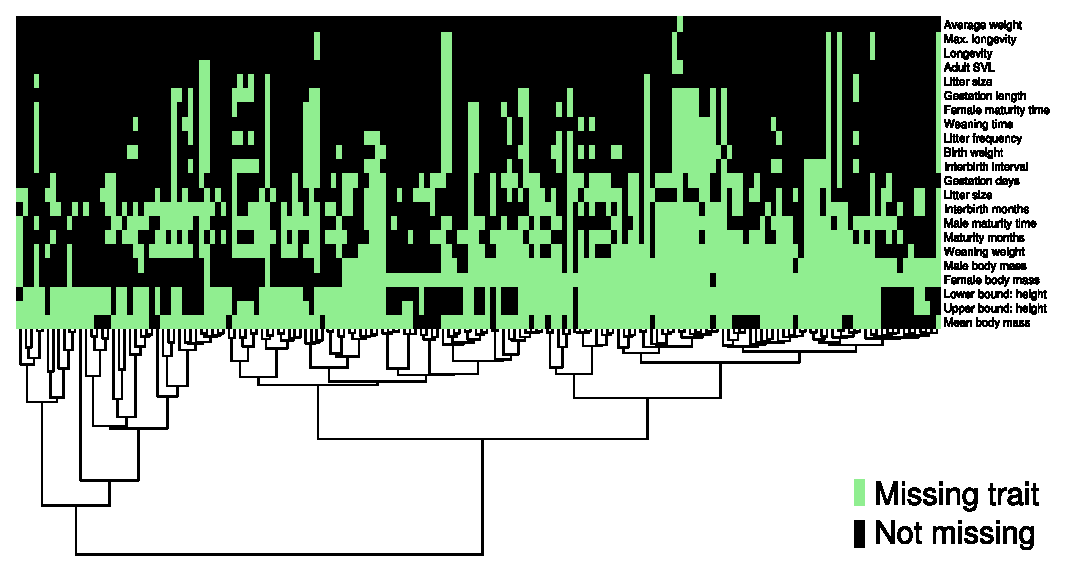
\includegraphics[width=\linewidth]{figs/ch5/missingness.pdf}
\caption[Missing trait map matched to the species level phylogeny]{Missing trait map matched to the species level phylogeny. The matrix in the upper half represents the trait data, with missing values shown in green. The columns of the matrix represent species, for which phylogenetic relationships are illustrated below. Rows that are mostly green represent poorly sampled traits, and columns that are mostly green represent poorly sampled species.}
\label{fig:missingness}
\end{figure}

\begin{figure}[ht]\centering
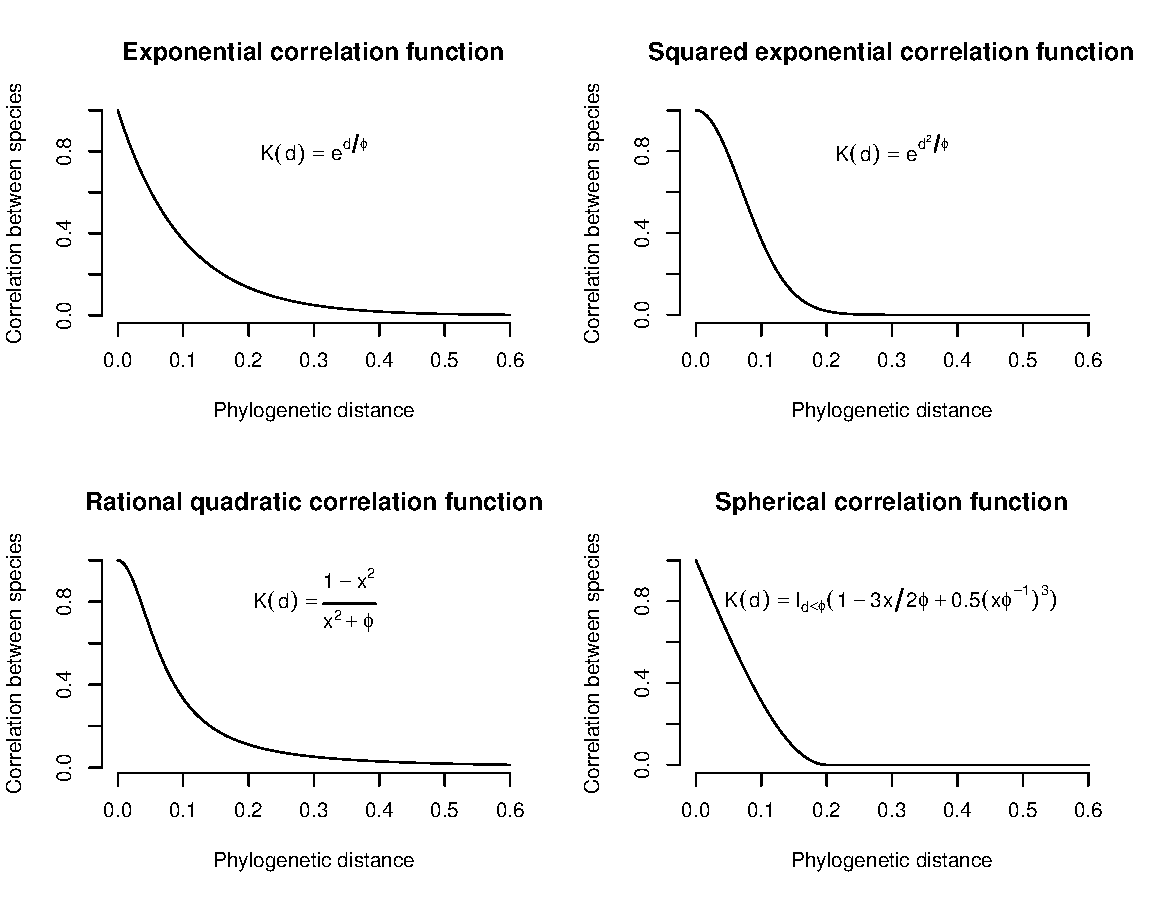
\includegraphics[width=\linewidth]{figs/ch5/cor_functions.pdf}
\caption[Correlation functions considered for the latent factors]{Correlation functions considered for the latent factors. The x-axis represents cophenetic distance between species, and the y axis represents the correlation induced by the function. Each function has one parameter $\phi$, but the shapes of the functions differ.}
\label{fig:cor_functions}
\end{figure}

\begin{figure}[ht]\centering
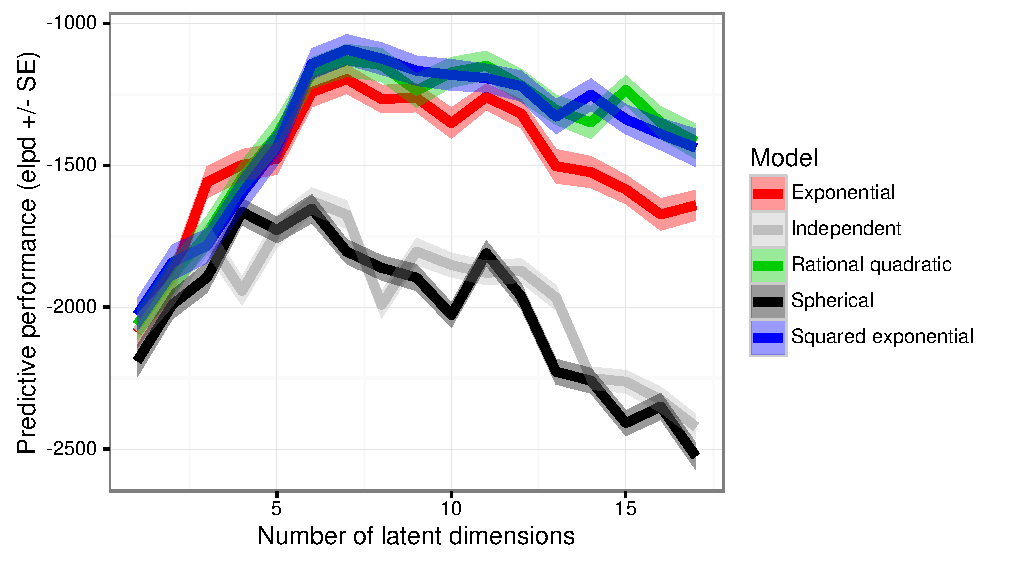
\includegraphics[width=\linewidth]{figs/ch5/model_comparisons.pdf}
\caption[Performance curves for models with varying phylogenetic correlation structures]{Performance curves for models with varying phylogenetic correlation structures (indicated by color), and latent factor dimensionality (shown in the x-axis). The y-axis is a measure of predictive performance for the model across all 10 folds. Specifically we show the expected log predictive density (elpd) plus and minus the standard error. High values of elpd indicate that the held out test data were consistent with the model predictions generated with the training data, and low values indicate that a model's predictions did not match the test data well.}
\label{fig:model_comparisons}
\end{figure}

\begin{figure}[ht]\centering
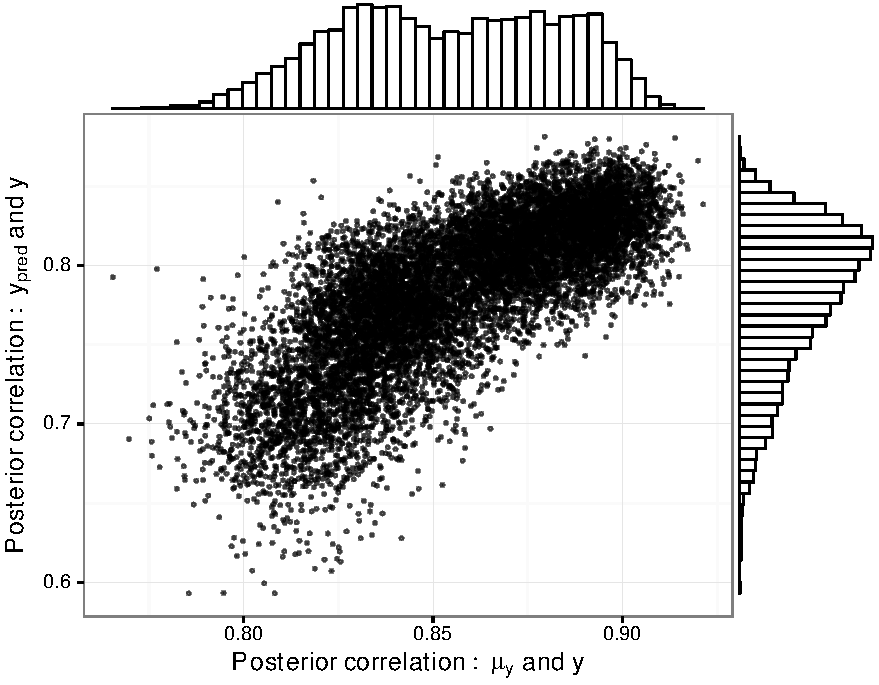
\includegraphics[width=\linewidth]{figs/ch5/rho.pdf}
\caption[Bivariate posterior distribution for the correlation between held-out values and posterior expected values]{Bivariate posterior distribution for the correlation between held-out values and posterior expected values (x-axis), and between the held-out values and the posterior predicted values (y-axis). Each point is a draw from the posterior distribution, and all draws are shown for each of the 10 folds. Marginal posterior histograms are shown for both quantities.}
\label{fig:rho}
\end{figure}

\begin{figure}[ht]\centering
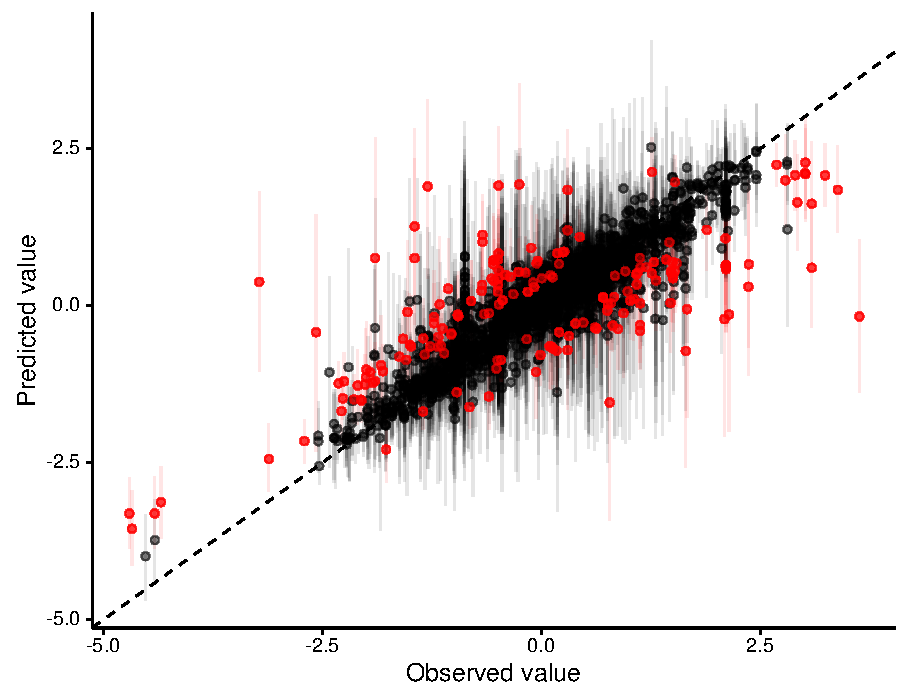
\includegraphics[width=\linewidth]{figs/ch5/predictions.pdf}
\caption[Observed (held out) values and model predictions]{Observed (held out) values and model predictions. Each point is a species trait, with the x position representing the true (scaled) value, and the y position of the point represents the posterior median prediction from a model with seven latent factors and a squared exponential phylogenetic correlation function. The vertical line segments represent 95\% credible intervals for the predicted trait values. The dashed line is a one to one line. If a point lies on this line, then the prediction was centered around the true value. Red indicates that the true held-out trait value was not in the 95\% prediction interval, and the red points have been plotted over the black points to highlight model misfit.}
\label{fig:predictions}
\end{figure}

\begin{figure}[ht]\centering
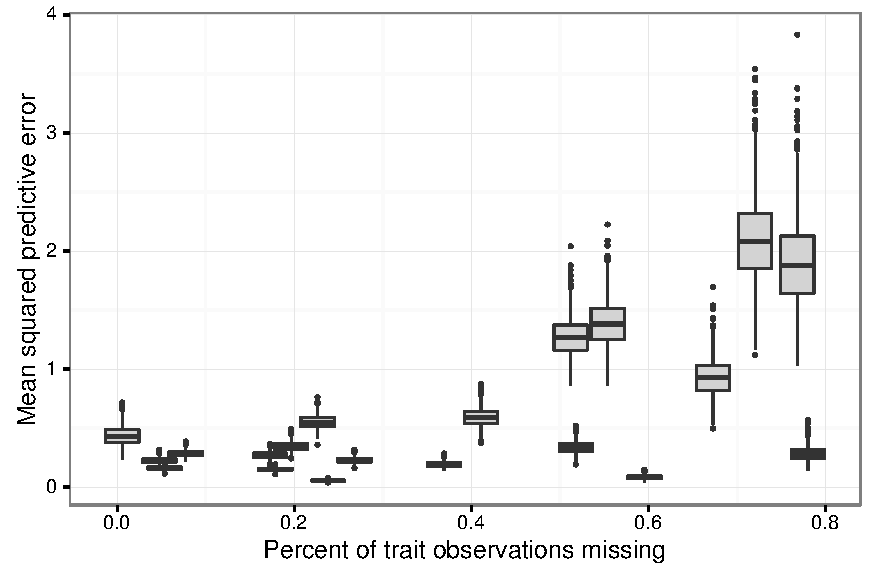
\includegraphics[width=\linewidth]{figs/ch5/mse.pdf}
\caption[Mean squared predictive error as a function of the number of trait observations]{Mean squared predictive error as a function of the number of trait observations. Each boxplot represents one trait. Well sampled traits are on the left half of the graph, and poorly sampled traits are on the right half. The midpoint in the box represents the posterior median, and the posterior quantiles are shown as the upper and lower portions of the box. Whiskers }
\label{fig:mse}
\end{figure}

\begin{figure}[ht]\centering
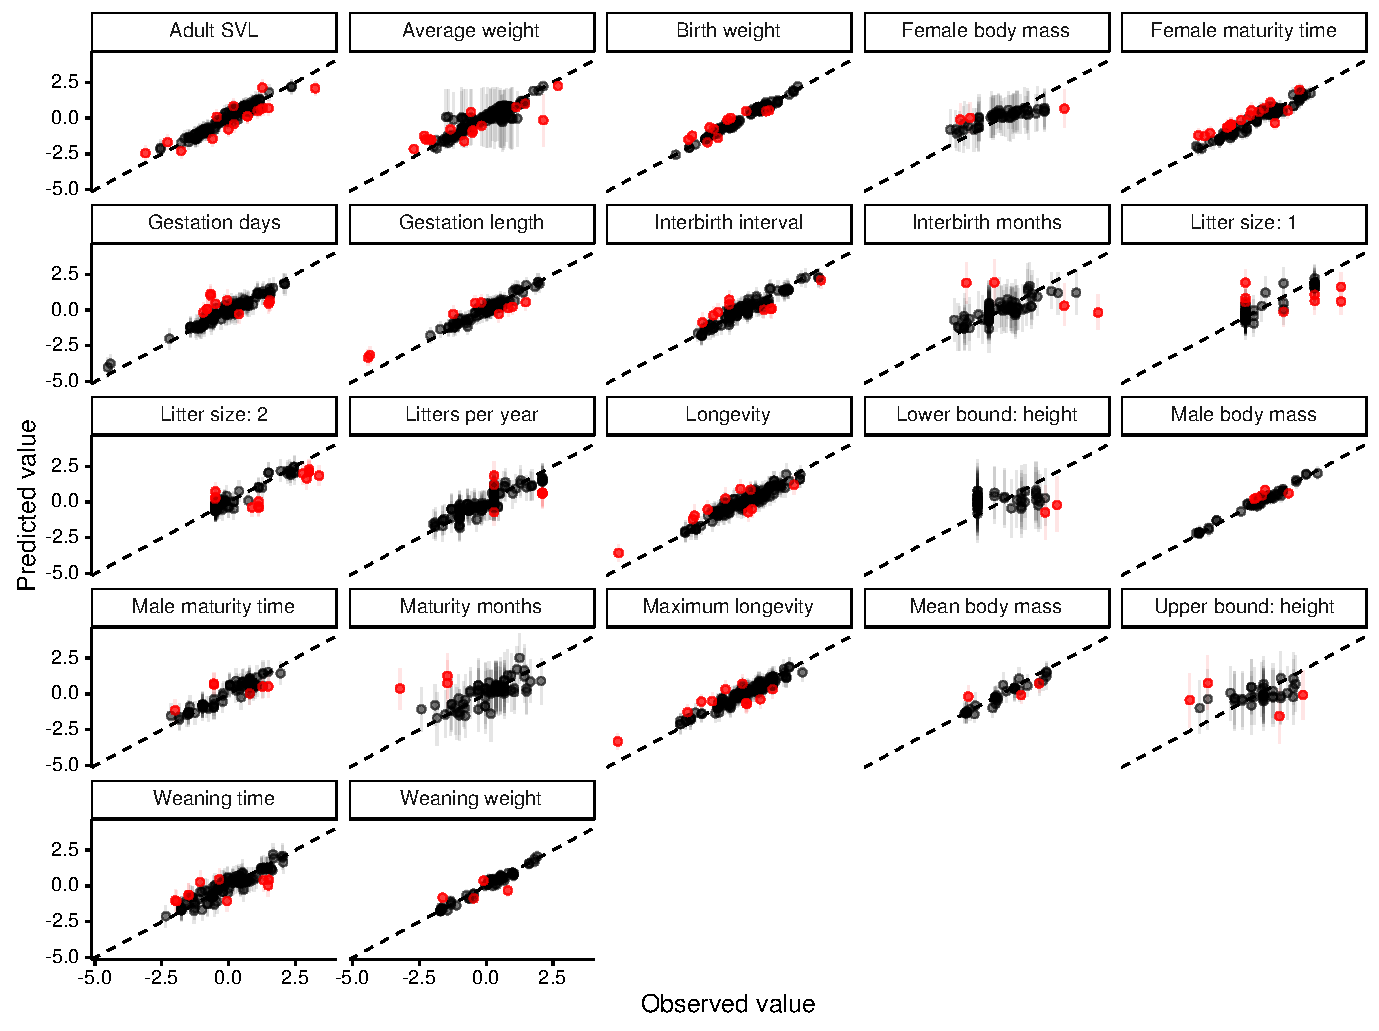
\includegraphics[width=\linewidth]{figs/ch5/by_trait.pdf}
\caption[Posterior predictions with 95\% prediction intervals, separated by trait]{Posterior predictions with 95\% prediction intervals, separated by trait. True values are on the x-axis, and the y-axis location of each point is the posterior median of the predicted value. Red indicates that the true held-out trait value was not in the 95\% prediction interval, and the red points have been plotted over the black points to highlight model misfit.}
\label{fig:by_trait}
\end{figure}
